\chapter{Mathematics}

\section{Formulas}

\subsection{Trigonometry}
\begin{align*}
\sin(v+w)&{}=\sin v\cos w+\cos v\sin w\\
\cos(v+w)&{}=\cos v\cos w-\sin v\sin w\\
\end{align*}
\begin{align*}
\tan(v+w)&{}=\dfrac{\tan v+\tan w}{1-\tan v\tan w}\\
\sin v+\sin w&{}=2\sin\dfrac{v+w}{2}\cos\dfrac{v-w}{2}\\
\cos v+\cos w&{}=2\cos\dfrac{v+w}{2}\cos\dfrac{v-w}{2}
\end{align*}
\[ (V+W)\tan(v-w)/2{}=(V-W)\tan(v+w)/2 \]
where $V, W$ are lengths of sides opposite angles $v, w$.
\begin{align*}
    a\cos x+b\sin x&=r\cos(x-\phi)\\
    a\sin x+b\cos x&=r\sin(x+\phi)
\end{align*}
where $r=\sqrt{a^2+b^2}, \phi=\operatorname{atan2}(b,a)$.

\section{Geometry}
\subsection{Triangles}
Side lengths: $a,b,c$ \\
Semiperimeter: $p=\dfrac{a+b+c}{2}$ \\
Area: $A=\sqrt{p(p-a)(p-b)(p-c)}$\\
Circumradius: $R=\dfrac{abc}{4A}$\\
Inradius: $r=\dfrac{A}{p}$\\
Length of median (divides triangle into two equal-area triangles): 
$m_a=\tfrac{1}{2}\sqrt{2b^2+2c^2-a^2}$\\
Length of bisector (divides angles in two): 
$s_a=\sqrt{bc\left[1-\left(\dfrac{a}{b+c}\right)^2\right]}$\\
Law of sines: 
$\dfrac{\sin\alpha}{a}=\dfrac{\sin\beta}{b}=\dfrac{\sin\gamma}{c}=\dfrac{1}{2R}$\\
Law of cosines: 
$a^2=b^2+c^2-2bc\cos\alpha$\\
Law of tangents: $\dfrac{a+b}{a-b}=\tan\dfrac{\alpha+\beta}{2}/\tan\dfrac{\alpha-\beta}{2}$ \\

\subsection{Quadrilaterals}
With side lengths $a,b,c,d$, diagonals $e, f$, diagonals angle $\theta$, area $A$ and
magic flux $F=b^2+d^2-a^2-c^2$:
\[ 4A = 2ef \cdot \sin\theta = F\tan\theta = \sqrt{4e^2f^2-F^2} \]
For cyclic quadrilaterals the sum of opposite angles is $180^\circ$,
$ef = ac + bd$, and $A = \sqrt{(p-a)(p-b)(p-c)(p-d)}$.

\subsection{Spherical coordinates}
\begin{center}
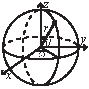
\includegraphics[width=25mm]{content/math/sphericalCoordinates}
\end{center}
\[\begin{array}{cc}
x = r\sin\theta\cos\phi & r = \sqrt{x^2+y^2+z^2}\\
y = r\sin\theta\sin\phi & \theta = \textrm{acos}(z/\sqrt{x^2+y^2+z^2})\\
z = r\cos\theta & \phi = \textrm{atan2}(y,x)
\end{array}\]

\section{Probability theory}
\subsection{Distributions}
\subsection{Markov chains}

\section{Derivatives / integrals}
\begin{align*}
	\dfrac{d}{dx}\arcsin x = \dfrac{1}{\sqrt{1-x^2}} &&& \dfrac{d}{dx}\arccos x = -\dfrac{1}{\sqrt{1-x^2}} \\
	\dfrac{d}{dx}\tan x = 1+\tan^2 x &&& \dfrac{d}{dx}\arctan x = \dfrac{1}{1+x^2} \\
	\int\tan ax = -\dfrac{\ln|\cos ax|}{a} &&& \int x\sin ax = \dfrac{\sin ax-ax \cos ax}{a^2} \\
	\int e^{-x^2} = \frac{\sqrt \pi}{2} \text{erf}(x) &&& \int xe^{ax}dx = \frac{e^{ax}}{a^2}(ax-1)
\end{align*}

\section{Combinatorial}

\subsection{Sums}
\[ 1+x+x^2+\ldots + x^n = \frac{x^{n+1}-1}{x-1} \]
\vspace{3pt}\\
\begin{align*}
1 + 2 + 3 + \ldots + n = \frac{n(n+1)}{2}\\
1^2 + 2^2 + 3^2 + \ldots + n^2 = \frac{n(2n+1)(n+1)}{6}\\
1^3 + 2^3 + 3^3 + \ldots + n^3 = \frac{n^2(n+1)^2}{4}\\
1^4 + 2^4 + 3^4 + \ldots + n^4 = \frac{n(n+1)(2n+1)(3n^2+3n-1)}{30}\\
\end{align*}
In general, we have 
\[ \sum_{i=1}^n n^m = \frac{1}{m+1} \sum_{k=0}^m \binom{m+1}{k} B_k \cdot (n+1)^{m+1-k} \]
EGF of Bernoulli numbers is $B(t)=\frac{t}{e^t-1}$ (FFT-able).
$B[0,\ldots] = [1, -\frac{1}{2}, \frac{1}{6}, 0, -\frac{1}{30}, 0, \frac{1}{42}, \ldots]$.
Bernoulli numbers satisfy the recursion
\[ B_n = \frac{-1}{n+1}\sum_{k=0}^{n-1}\binom{n+1}{k}B_k \]
\vspace{3pt}\\
\begin{align*}
\sum_{k=1}^n \binom{n}{k}^2 = \binom{2n}{n}\\
\sum_{k=m}^{n} \binom{k}{m} = \binom{n+1}{m+1}\\
\sum_{k=0}^{n} \binom{m+k-1}{k} = \binom{n+m}{n}\\
\sum_{k=0}^n \binom{a}{k}\binom{b}{n-k} = \binom{a+b}{n} \:\:\: (a+b \geq n)\\
\end{align*}

\subsection{Paths / bracket sequences}
Catalan numbers: ${C_n = 1, 1, 2, 5, 14, 42, 132, 429, 1430, 4862, 16796, 58786, \dots}$
\[ C_n=\frac{1}{n+1}\binom{2n}{n}= \binom{2n}{n}-\binom{2n}{n+1} = \frac{(2n)!}{(n+1)!n!} \]
\[ C_0=1,\ C_{n+1} = \frac{2(2n+1)}{n+2}C_n,\ C_{n+1}=\sum C_iC_{n-i} \]
\begin{itemize}[noitemsep]
    \item binary trees with with $n+1$ leaves (0 or 2 children).
    \item ordered trees with $n+1$ vertices.
    \item ways a convex polygon with $n+2$ sides can be cut into triangles by connecting vertices with straight lines.
    \item permutations of $[n]$ with no 3-term increasing subseq.
\end{itemize}
Narayana numbers: $N(n,k) = \frac{1}{n}\binom{n}{k}\binom{n}{k-1}$. The following hold:
\[ $N(n,k)=N(n,n-k+1)$, \ N(n,1) + N(n,2) + \ldots + N(n,k) = C(n) \]
\begin{itemize}[noitemsep]
    \item rooted trees with $n+1$ vertices and $k$ leaves.
    \item balanced bracket sequences with $2n$ brackets and $k$ peaks.
\end{itemize}

\section{Generating functions}
If $p$ is the EGF of sets with some property, then $e^p$ is the EGF of sets partitioned into sets with the property.\\
\vspace{3pt}\\
\textbf{Cycles} Let $g_S(n)$ be the number of $n$-permutations whose cycle lengths all belong to the set $S$. Then
\[ \sum_{n=0} ^\infty g_S(n) \frac{x^n}{n!} = \exp\left(\sum_{n\in S} \frac{x^n} {n} \right) \]

\subsection{Stirling numbers}

